\documentclass{beamer}
%\usetheme{Madrid}
%\usetheme{Berlin}
%\usepackage{german}
%\usepackage[latin1]{inputenc}
%\usepackage[T1]{fontenc}
%\mode<presentation>
 %{
 \usetheme{Madrid}
 \setbeamercolor*{palette primary}{use=structure,fg=black,bg=p7408C}
 \setbeamercolor*{palette secondary}{use=structure,fg=black,bg=p7406U}
 \setbeamercolor*{palette tertiary}{use=structure,fg=black,bg=p716C}
 %}
 
 \definecolor{p7408C}{HTML}{F6BE00}
  \definecolor{p7406U}{HTML}{FCB315}
 \definecolor{pyelloy}{HTML}{F6C100}
 \definecolor{p716C}{HTML}{F17C0E}
 
  \definecolor{p8C}{HTML}{A19589}
 \setbeamercolor{itemize item}{fg=p8C} % all frames will have red bullets
 \setbeamertemplate{itemize item}[triangle]
 \setbeamertemplate{itemize subitem}{\color{p7408C}$\blacktriangleright$}

\setbeamercolor{block title}{bg=p7408C,fg=black}

\usepackage{etex}
\usepackage{tikz,pgfplots}
\usepackage{picture}

%\usepackage{german}
%\usepackage[latin1]{inputenc}
\usepackage[T1]{fontenc}
\usepackage{booktabs}
\usepackage{graphicx}
\usepackage{epsfig}
\usepackage{changebar}
\usepackage{amsmath}
\usepackage{mathtools}
\usepackage[T1]{fontenc}
\usepackage[ansinew]{inputenc}
\usepackage{setspace}
\usepackage{multicol}
\usepackage{multirow}
\usepackage{dcolumn}
\usepackage{color}
\usepackage{colortbl}
\definecolor{lightgray}{gray}{0.8}
\definecolor{lightblue}{rgb}{0.8,0.8,0.8}
\usepackage{hyperref}
\usepackage{xcolor} 
\usepackage{array} 
\usepackage{subfig}
\usepackage{makecell}
\usetikzlibrary{arrows,positioning} 


\graphicspath{{/Users/jupiter/Dropbox/elements/coala/graphs/}{../../../../Dropbox/elements/spatialrebels/graphs/}{../../../../Dropbox/elements/spatialrebels/graphspres/}}



\begin{document}

\title[UCL]
{
Violent actors and their interactions. Forecasting conflict dynamics}
\author[GCRI]
{
Nils W. Metternich \\[3ex]
\footnotesize{\emph{COnflict Analysis LAb (COALA)}}\\
\textbf{Funded by the Economic and Social Research Council (UK)}}
\institute[]
{		Department of Political Science\\
		University College London\\
		n.metternich@ucl.ac.uk\\[4ex]
		}

\date{June 12, 2018}

\begin{frame}
\titlepage
\end{frame}

\begin{frame}{The golden triangle?}
\begin{itemize}
\item Promise 1: Disaggregation instead of aggregation. 
\item Promise 2: Non-linearity vs. linearity; Non-parametric vs. parametric
\item Promise 3: (Strategic) Interdependence instead of independence  
\end{itemize}
\end{frame}


\begin{frame}{Predictive turn in conflict studies}
\begin{minipage}{2.1in}
\begin{tiny}
\begin{itemize}
\item Gurr and Lichbach, 1986
\item O'brien, 2002
\item Schrodt, 2006
\item Goldstone et al., 2010
\item Ward, 2010
\item Weidmann and Ward, 2010
\item Schneider, Gleditsch and Carey, 2011
\end{itemize}
 \end{tiny}
\end{minipage}
\begin{minipage}{2.5in}
\begin{tiny}
\begin{itemize}
\item De Mesquita, 2011
\item Ward et al., 2013
\item Gleditsch and Ward, 2013
\item Hegre et al., 2013
\item Bell et al., 2013
\item Brandt, Freeman and Schrodt, 2014
\item Muchlinski et al., 2016
\end{itemize}
 \end{tiny}
\end{minipage}
\end{frame}

\begin{frame}{Interdependence turn}
\begin{center}
Monadic analysis $\rightarrow$ Dyadic analysis $\rightarrow$ Network analysis\\
\includegraphics[scale=0.45,angle=90]{network_104b.pdf}\\
\tiny{
\begin{tabular}{lll}
Collier and Hoeffler (2000) & Cunningham et al. (2009) & Ward et al. (2013) \\
Fearon and Laitin (2003)   & Wucherpfennig et al. (2012) & Metternich et al. (2013)  \\
Bates et al. (2005)    & Bapat and Bond (2012) & Starr and Most (1983)     \\
Cunningham (2006)& Walter (2009) & Maoz (2010)\\
Gleditsch et al. (2002) & Bakke et al. (2012) & Larson and Lewis (2017)\\
Hegre et al. (2001) & Steinwand (2011) & Chyzh (2016)\\
& Cunningham (2013) & Franzese and Hays (2008) \\
\end{tabular}}
\end{center}
\end{frame}


\begin{frame}
\centering
\begin{table}
\caption{Ideal types of analyzing independence in conflicts.}
\label{tab:4by4}
\scalebox{0.72}{%
\begin{tabular}{l|c|l|l}
Type &Representation& Rebels' Utility& $y= \hdots +\epsilon$\\
\hline
Aggregate &
\begin{tikzpicture}
\draw [fill=gray,gray] (0,0) circle [radius=0.1];
\draw [fill=white,white] (2,0) circle [radius=0.1];
\draw [fill=white,white] (-2,0) circle [radius=0.1];
\draw [fill=white,white] (0,0.75) circle [radius=0.1];
\draw [fill=white,white] (0,-0.75) circle [radius=0.1];
\end{tikzpicture}
& $U_{i}(X)$ & $X\beta$ \\
\hline 
Dyadic & 
\begin{tikzpicture}
\draw [fill=gray,gray] (0,0) circle [radius=0.1];
\draw [fill] (1,0) circle [radius=0.1];
\draw [fill=white,white] (2,0) circle [radius=0.1];
\draw [fill=white,white] (-2,0) circle [radius=0.1];
\draw [<->] (0.15,0) -- (0.85,0);
\draw [fill=white,white] (0,0.75) circle [radius=0.1];
\draw [fill=white,white] (0,-0.75) circle [radius=0.1];
\end{tikzpicture}
& $U_{i}(X,Z)$ & $X\beta$+$Z\zeta$ \\
\hline 
K-dyads & 
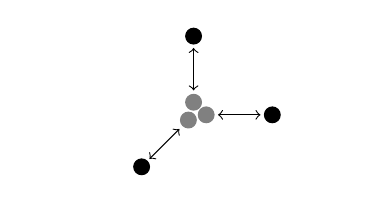
\begin{tikzpicture}
\draw [fill=gray,gray] (0,.16) circle [radius=0.1];
\draw [fill=gray,gray] (.16,0) circle [radius=0.1];
\draw [fill=gray,gray] (-.066,-.066) circle [radius=0.1];
\draw [fill] (0,1) circle [radius=0.1];
\draw [fill] (-0.66,-0.66) circle [radius=0.1];
\draw [fill] (1,0) circle [radius=0.1];
\draw [fill=white,white] (2,0) circle [radius=0.1];
\draw [fill=white,white] (-2,0) circle [radius=0.1];
\draw [<->] (0.31,0) -- (0.85,0);
\draw [<->] (0,0.31) -- (0,0.85);
\draw [<->] (-0.18,-0.18) -- (-0.56,-0.56);
\end{tikzpicture}

& $U_{i}(X,Z,K)$ & $X\beta$+$Z\zeta$+$K\kappa$ \\
\hline 
K-adic & 
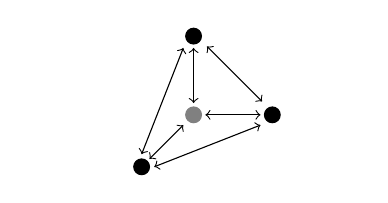
\begin{tikzpicture}
\draw [fill=gray,gray] (0,0) circle [radius=0.1];
\draw [fill] (0,1) circle [radius=0.1];
\draw [fill] (-0.66,-0.66) circle [radius=0.1];
\draw [fill] (1,0) circle [radius=0.1];
\draw [fill=white,white] (2,0) circle [radius=0.1];
\draw [fill=white,white] (-2,0) circle [radius=0.1];
\draw [<->] (0.15,0) -- (0.85,0);
\draw [<->] (0,0.15) -- (0,0.85);
\draw [<->] (-0.13,-0.13) -- (-0.56,-0.56);
\draw [<->] (-0.66,-0.5) -- (-.13,0.85);
\draw [<->] (-0.5,-0.66) -- (0.85,-.13);
\draw [<->] (0.17,.87) -- (.87,.17);
\end{tikzpicture}
& $U_{i}(X,Z,Y_{j},W)$ & $X\beta$+$Z\zeta$+$K\kappa$+$\rho Wy$ \\
\end{tabular}}
\end{table}
\end{frame}

\begin{frame}{Example 1}{Metternich, Minhas, and Ward, 2017}
\includegraphics[width=1\textwidth]{../../../../Desktop/contagion_map.png}
\end{frame}

\begin{frame}{Example 1}{Metternich, Minhas, and Ward, 2017}
\includegraphics[width=1\textwidth]{../../../../Desktop/contagion_prediction.png}
\end{frame}


\begin{frame}{Example 2}{Metternich and Wucherpfennig, working paper}
\begin{figure}[ht!]
\centering
\includegraphics[scale=0.35]{overlap_cases.pdf}
\caption{Rebel organization activity during selected UCDP armed conflicts.
%: Examples Chad $(UCDP ID=91)$, Congo $(UCDP ID=214)$, Uganda $(UCDP ID=118)$, and Guatemala $(UCDP ID=36)$. 
Each row represents a separate rebel organization as defined by a unique UCDP  $SideB$ for each rebel organization.}
\label{fig:example}
\end{figure}
\end{frame}

\begin{frame}{Model fit and insample prediction}
\begin{figure}[h!]
\begin{center}
\subfloat[Predicted densities]{\includegraphics[width=4cm]{twobytwoa.pdf}}
\subfloat[Relative advantage]{\includegraphics[width=4cm]{twobytwod.pdf}}
\subfloat[Case-wise comparison]{\includegraphics[width=4cm]{twobytwob.pdf}}
\caption{Model fit and insample prediction assessment comparing Model~1 (k-dyadic Weibull controlling for the number of rebel organizations) and Model~3 (spatial k-adic Weibull including the number of rebel organizations). In all panels orange refers to Model 1, while purple pertains to Model~3.}
\end{center}
\end{figure}
\end{frame}


\begin{frame}{Example 3}{Metternich et al., conference paper }
RebelCast:
\begin{itemize}
\item Makes predictions for rebel organizations (disaggregation)
\item Supported by machine learning ensembles
\item With a focus on interdependent actors
\end{itemize}
\end{frame}

\begin{frame}{Conclusion}{Suggestions for GCRI}
\begin{itemize}
\item Disaggregate (but needs to be operationally relevant)
\item Allow for non-linear, non-parametric processes
\item Allow for interdependencies between actors (governments, states, rebel organizations etc)
\end{itemize}
\end{frame}


\end{document}


\begin{frame}{Predicting escalation of conflicts is difficult}
\begin{figure}
\includegraphics[scale=0.5]{Rplot011.png}
\caption{Predictions for continuous escalation measure}
\end{figure}
\end{frame}

\begin{frame}{Outcome variable}{Challenge of measuring escalation}
\begin{figure}
\includegraphics[scale=0.5]{extreme_values_quantiles.png}
\caption{Creating categorial variable}
\end{figure}
\end{frame}

\begin{frame}{Predicting escalation of conflict}
\begin{figure}
\includegraphics[scale=0.5]{Rplot01.png}
\caption{Predictions for categorial escalation measure}
\end{figure}
\end{frame}

\begin{frame}
\begin{table}
\caption{RF with dispersion-based categories}
\centering
\scalebox{0.75}{
\begin{tabular}[t]{l|r|r|r|r|r}
\hline
  & Sensitivity & Specificity & Pos Pred Value & Neg Pred Value & Balanced Accuracy\\
\hline
Class: 0 & 0.9939446 & 0.7546296 & 0.9559068 & 0.9588235 & 0.8742871\\
\hline
Class: 1 & 0.6903226 & 0.9806902 & 0.8199234 & 0.9613371 & 0.8355064\\
\hline
Class: 2 & 0.5655738 & 0.9961861 & 0.8734177 & 0.9801126 & 0.7808799\\
\hline
\end{tabular}}

\caption{Strong but naive classifier (only lagged DV)}
\centering
\scalebox{0.75}{
\begin{tabular}[t]{l|r|r|r|r|r}
\hline
  & Sensitivity & Specificity & Pos Pred Value & Neg Pred Value & Balanced Accuracy\\
\hline
Class: 0 & 0.9566755 & 0.7706856 & 0.9570986 & 0.7688679 & 0.8636805\\
\hline
Class: 1 & 0.6072607 & 0.9500420 & 0.6072607 & 0.9500420 & 0.7786514\\
\hline
Class: 2 & 0.6583333 & 0.9836257 & 0.6528926 & 0.9840094 & 0.8209795\\
\hline
\end{tabular}}
\end{table}
\end{frame}

\begin{frame}{Next steps}
\begin{itemize}
\item Implement further ML approaches
\item Leverage heterogeneity through EBMAs
\item Rebel organization implementation
\end{itemize}
\end{frame}





\begin{frame}
\begin{table}
\caption{Estimates for the main fighting duration models in accelerated failure time format. Standard errors are provided in parenthesis. Outcome variable is the fighting duration of rebel organizations measured in days.}
\begin{center}
\scalebox{0.5}{
\begin{tabular}{l D{.}{.}{4.5}@{} D{.}{.}{4.5}@{} D{.}{.}{4.5}@{} D{.}{.}{4.5}@{} D{.}{.}{4.5}@{} }
\hline
                         & \multicolumn{1}{c}{Veto Model} & \multicolumn{1}{c}{Spatial Model} & \multicolumn{1}{c}{Spatial Veto Model} & \multicolumn{1}{c}{Secession Model} & \multicolumn{1}{c}{Non-Secession Model} \\
\hline
Intercept                & 7.28^{***}  & 7.11^{***}  & 7.11^{***}  & 8.46^{***}  & 7.14^{***}  \\
                         & (0.30)      & (0.30)      & (0.30)      & (0.51)      & (0.33)      \\
Time until Entry$_{log}$ & 0.01        & -0.00       & -0.00       & -0.07^{*}   & 0.03        \\
                         & (0.03)      & (0.02)      & (0.02)      & (0.04)      & (0.03)      \\
Splinter                 & 0.12        & -0.04       & -0.03       & 0.41        & -0.13       \\
                         & (0.26)      & (0.26)      & (0.26)      & (0.42)      & (0.33)      \\
Alliance                 & -0.25       & -0.55^{*}   & -0.56^{*}   & -0.04       & -0.69^{*}   \\
                         & (0.31)      & (0.31)      & (0.31)      & (0.67)      & (0.36)      \\
Previous Victory         & -0.03       & -0.07       & -0.06       & 0.71        & -0.16       \\
                         & (0.10)      & (0.10)      & (0.10)      & (0.61)      & (0.11)      \\
Previous Agreement       & -0.07       & -0.08       & -0.09       & 0.12        & -0.06       \\
                         & (0.10)      & (0.09)      & (0.09)      & (0.47)      & (0.10)      \\
Legal Political Wing     & -0.54^{**}  & -0.55^{**}  & -0.54^{**}  & -1.13^{***} & -0.44       \\
                         & (0.22)      & (0.22)      & (0.22)      & (0.34)      & (0.28)      \\
Rebel Strength           & -0.39^{***} & -0.36^{***} & -0.36^{***} & -0.56^{**}  & -0.43^{***} \\
                         & (0.12)      & (0.12)      & (0.12)      & (0.24)      & (0.14)      \\
Veto                     & 0.25^{*}    &             & -0.10       & -0.10       & 0.05        \\
                         & (0.14)      &             & (0.16)      & (0.33)      & (0.17)      \\
Secession                & 0.51^{**}   & 0.52^{***}  & 0.51^{***}  &             &             \\
                         & (0.20)      & (0.20)      & (0.20)      &             &             \\
Scale$_{log}$            & 0.49^{***}  & 0.47^{***}  & 0.47^{***}  & 0.30^{***}  & 0.52^{***}  \\
                         & (0.04)      & (0.04)      & (0.04)      & (0.08)      & (0.05)      \\
$\rho$                   &             & 0.13^{***}  & 0.14^{***}  & 0.06        & 0.13^{***}  \\
                         &             & (0.03)      & (0.03)      & (0.05)      & (0.03)      \\
\hline
Log-Likelihood           & -791.91     & -782.25     & -782.05     & -202.29     & -575.20     \\
N                        & 379         & 379         & 379         & 107         & 272         \\
\hline
\multicolumn{6}{l}{\scriptsize{$^{***}p<0.01$, $^{**}p<0.05$, $^*p<0.1$}}
\end{tabular}
}
\label{tab:estSepAll}
\end{center}
\end{table}
\end{frame}


\begin{frame}
\begin{table}
\caption{Estimates for the main fighting duration models in accelerated failure time format. Standard errors are provided in parenthesis. Outcome variable is the fighting duration of rebel organizations measured in days.}
\begin{center}
\scalebox{0.6}{
\begin{tabular}{l D{.}{.}{4.5}@{} D{.}{.}{4.5}@{} D{.}{.}{4.5}@{} D{.}{.}{4.5}@{} D{.}{.}{4.5}@{} }
\hline
                         & \multicolumn{1}{c}{Veto Model} & \multicolumn{1}{c}{Spatial Model} & \multicolumn{1}{c}{Spatial Veto Model} & \multicolumn{1}{c}{Secession Model} & \multicolumn{1}{c}{Non-Secession Model} \\
\hline

$\rho$                   &             & 0.13^{***}  & 0.14^{***}  & 0.06        & 0.13^{***}  \\
                         &             & (0.03)      & (0.03)      & (0.05)      & (0.03)      \\
\hline
Log-Likelihood           & -791.91     & -782.25     & -782.05     & -202.29     & -575.20     \\
N                        & 379         & 379         & 379         & 107         & 272         \\
\hline
\multicolumn{6}{l}{\scriptsize{$^{***}p<0.01$, $^{**}p<0.05$, $^*p<0.1$}}
\end{tabular}
}
\label{tab:estSepAll}
\end{center}
\end{table}
\end{frame}

\begin{frame}{Strategic perspective}
\begin{block}{Definition}
A theoretical approach that views individuals [actors] as choosing their actions by taking into account the \alert{anticipated actions and responses of others} with the intention of maximizing their own welfare (B. de Mesquita 2014, 535).
\end{block}
\end{frame}

\begin{frame}{N-Player Network Game Theoretic Model}
Consideration 1:
\begin{itemize}
\item Rebel organizations in multi-actor conflicts share the objective of either:
\begin{itemize}
\item overthrowing the government
\item gaining regional autonomy/secession
\end{itemize}
\item E.g., ousting the regime of Muammar Gaddafi or Palestinian independence
\item[]
\item Benefits of incompatibilities like democratization, respect for human rights, right for self-determination, end to alien rule are not limited to any particular opposition group
\item Non-excludability and non-rivalry
\item[$\rightarrow$] \alert{Public goods}
\end{itemize}
\end{frame}

\begin{frame}{Public Goods Game}
Following Bramoull\'{e}, Kranton and D'amours 2014:
\begin{align}
U_{i}(y_i,\mathbf{y_j},\delta,\mathbf{W})= b_{i}\left(y_{i} +  \delta \sum_{j} w_{ij}y_{j}\right) - c_{i}y_{i} \label{EU_subst}
\end{align}
Best response:
\begin{align}
\label{best:response}
y_{i}^{*}&= \bar{y_{i}}- \delta \sum_{j} w_{ij}y_{j} &\text{if} \hspace{2mm} \delta \sum_{j} w_{ij}y_{j}<\bar{y_{i}}\\ \notag
y_{i}^{*}&=0 &\text{if} \hspace{2mm} \delta \sum_{j} w_{ij}y_{j}\geq \bar{y_{i}}
\end{align} 
\end{frame}

\begin{frame}{N-Player Network Game Theoretic Model}
Consideration 2:
\begin{itemize}
\item Rebel organizations compete against one another
\begin{itemize}
\item Rebel-rebel violence (Fjelde  \& Nillson 2012)
\item Dual-contest (Cunningham, Bakke \& Seymour 2012)
\item Fragmentation/splintering
\end{itemize}
\end{itemize}
\end{frame}


\begin{frame}{Theoretical Model 2}
Rivalrous Good Network Game
\begin{equation}
U_{i}(y_i,\mathbf{y_j},\delta,\mathbf{W})= b_{i}\left(y_{i} -  \gamma \sum_{j} w_{ij}y_{j} \right) - c_{i}y_{i} \label{EU_comp}
\end{equation}
Best response
\begin{equation}
y_{i}^{*}= \bar{y_{i}}+ \delta \sum_{j} w_{ij}y_{j} 
\label{best_comp}
\end{equation} 
\end{frame}


\begin{frame}{Combined Model}
\begin{align}
U_{i}(y_i,\mathbf{y_j},\delta,\mathbf{W})&= b_{i}\left(y_{i} +  \delta \sum_{j} w_{ij}y_{j} -  \gamma \sum_{j} w_{ij}y_{j} \right) - c_{i}y_{i} \label{EU_comp}\\
% &= b_{i}\left(y_{i} +  (\delta- \gamma) \sum_{j} w_{ij}y_{j} \right) - c_{i}y_{i}\\
%U_{i}(y_i,\mathbf{y_j},\delta,\mathbf{W}) 
&= b_{i}\left(y_{i} +  \rho \sum_{j} w_{ij}y_{j} \right) - c_{i}y_{i}\label{EU_joint}
\end{align}
where $\rho =\delta-\gamma$.
\end{frame}

\begin{frame}{Best response functions}
\begin{figure}[h!]
\centering
\includegraphics[scale=0.6]{effortsSim3.pdf}
\end{figure}
\end{frame}

\begin{frame}
\frametitle{Non-aligned fighting durations}
\begin{center}
\includegraphics[scale=0.35]{enterfight.pdf}
\end{center}
\end{frame}

\begin{frame}{Model fit and insample prediction}
\begin{figure}
\begin{center}
%\subfigure[Absolute deviation]{\includegraphics[scale=0.4]{twobytwoc.pdf}}
\subfloat[Predicted densities for separatist conflict sample.]{\includegraphics[width=4cm]{twobytwoaS.pdf}}
\subfloat[Relative advantage for separatist conflict sample.]{\includegraphics[width=4cm]{twobytwodS.pdf}}
\subfloat[Case-wise comparison for separatist conflict sample.]{\includegraphics[width=4cm]{twobytwobS.pdf}} 
\end{center}
\end{figure}
\end{frame}



\begin{frame}{Model fit and insample prediction}
\begin{figure}
\begin{center}
%\subfigure[Absolute deviation]{\includegraphics[scale=0.4]{twobytwoc.pdf}}
\subfloat[Predicted densities for non-separatist conflict sample.]{\includegraphics[width=4cm]{twobytwoaNS.pdf}}
\subfloat[Relative advantage for non-separatist conflict sample.]{\includegraphics[width=4cm]{twobytwodNS.pdf}}
\subfloat[Case-wise comparison for non-separatist conflict sample.]{\includegraphics[width=4cm]{twobytwobNS.pdf}}
\end{center}
\end{figure}
\end{frame}

\begin{frame}{ICEWS}
\centering
\includegraphics[scale=0.1]{DRC.png}
\end{frame}


\begin{frame}{Challenges made for machine learning}
\begin{itemize}
\item Theoretical limitatations
\item P>N
\item Non-linear processes
\item Higher order interactions
\end{itemize}
\end{frame}

\begin{frame}{Idea behind trees}
\begin{itemize}
\item Given sample $N$ and regressors $X_{i}$, we sequentially partition the covariate space into subspaces in a way that reduces the sum of squared residuals as much as possible. 


\item Suppose, we have two covariates $X_{1}$ and $X_{2}$.

\item We can split the sample by $X{_1}<c$ versus $X{_1} \leq c$, or $X{_2}<c$ versus $X{_2} \leq c$. 

\item We look for the split that minimizes the sum of squared residuals. 

\item If a variable partitions the data perfectly sum of squared residuals equals 0

\item Then we consider the next split for each of the two subsets. 

\item Stop once the reduction in the sum of squared residuals is below some threshold. 

\end{itemize}
\end{frame}

\begin{frame}{Random forests}
Non-parametric statistical learning approach
\begin{enumerate}
\item Draw $B$ bootstrap samples from the original data.
\item Grow a tree for each bootstrapped data set. At each node of the tree, randomly select $p$ number of predictors for splitting on. 
\begin{itemize}
\item A node is split on that predictor which maximizes survival differences across daughter nodes.
\end{itemize}
\item Grow the tree to full size under the constraint that a terminal node should have no less than $n$ unique observations.
\item Calculate an ensemble-wide sum of squared residuals by combining information from $B$ trees.
%\item Compute an out-of-bag (OOB) error rate for the forest ensemble, derived by using $b$ trees, where $b=1, \dots, B$.
\end{enumerate}
\end{frame}

\begin{frame}{Multi-actor Conflicts}
\begin{figure}[b!]
\centering
\includegraphics[scale=0.4]{barplot.pdf}
\caption{Number of rebel organizations in one UCDP conflict. Left panel illustrates difference between single and multi-actor conflicts. Right panel provides insights to the actual number of rebel organizations in these conflicts. 81 UCDP armed conflicts are single actor conflicts, 72 conflicts involve multiple parties and there exists a notable variation in how many rebel organizations participate in multi-actor conflicts.}
\label{fig:bar}
\end{figure}
\end{frame}




